\documentclass[10pt,twocolumn,letterpaper]{article}

\usepackage{iccv}
\usepackage{times}
\usepackage{epsfig}
\usepackage{graphicx}
\usepackage{subfigure}
\usepackage{amsmath}
\usepackage{amssymb}
\usepackage{multirow}
\usepackage{algorithm}
\usepackage{algpseudocode}

\renewcommand{\algorithmicrequire}{\textbf{Input:}} % Use Input in the format of Algorithm
\renewcommand{\algorithmicensure}{\textbf{Output:}} % Use Output in the format of Algorithm


% Include other packages here, before hyperref.

% If you comment hyperref and then uncomment it, you should delete
% egpaper.aux before re-running latex.  (Or just hit 'q' on the first latex
% run, let it finish, and you should be clear).
\usepackage[pagebackref=true,breaklinks=true,letterpaper=true,colorlinks,bookmarks=false]{hyperref}

% \iccvfinalcopy % *** Uncomment this line for the final submission

\def\iccvPaperID{****} % *** Enter the ICCV Paper ID here
\def\httilde{\mbox{\tt\raisebox{-.5ex}{\symbol{126}}}}

% Pages are numbered in submission mode, and unnumbered in camera-ready
\ificcvfinal\pagestyle{empty}\fi
\begin{document}

%%%%%%%%% TITLE
\title{Discrimination of ADHD children based on Deep Bayesian Network}

\author{Junyu Hao\\
Department of Computer Technology\\
Tongji University\\
Shanghai, China\\
{\tt\small haojunyu2012@gmail.com}
% For a paper whose authors are all at the same institution,
% omit the following lines up until the closing ``}''.
% Additional authors and addresses can be added with ``\and'',
% just like the second author.
% To save space, use either the email address or home page, not both
\and
Lianghua He\\
Department of Computer Science and Technology\\
Tongji University\\
Shanghai, China\\
{\tt\small helianghua@tongji.edu.cn}
}

\maketitle
%\thispagestyle{empty}


%%%%%%%%% ABSTRACT
\begin{abstract}
   Attention deficit hyperactivity disorder (ADHD) is a threat for the public health all the time, so the effective discrimination of it is significant and meaningful. In current research, Functional Magnetic Resonance Imaging (fMRI) data has become a popular tool for the analysis of ADHD. In this paper, we introduce the Deep Bayesian Network, a combination of Deep Belief Network and Bayesian Network, to classify the ADHD children from the normal. In Deep Bayesian Network, The Deep Belief Network is applied to  normalize and reduce dimension of the fMRI data in every brodmann area. And the Bayesian Network is used to extract the feature of relationships between several well-performed brain areas by structure learning. According to the information of structure and probability in Bayesian Network, we predicted the subjects as control,combined ,inattentive or hyperactive using SVM classifier. The final results perform better than using single Deep Belief Network and the best results in ADHD-200 competition. 

\end{abstract}

%%%%%%%%% BODY TEXT
\section{Introduction}
Attention deficit hyperactivity disorder(ADHD) is among the most common psychiatric disorders of childhood that persists into adulthood in the majority of cases\cite{1}. According to American Psychiatric Association's Diagnostic and Statistical Manual, the prevalence of ADHD in the whole world is approximately 5\%, especially in the United States the prevalence among 8 to 15-years-olds reaches to 8.7\% during the past years. Therefore, the methods of diagnosing the ADHD are in urgent need.
 
 
 
As an excellent method of measuring brain activation, fMRI
signals\cite{2} are studied to classify ADHD. Shengfu Liang et al.\cite{3} utilizes the LDA classifier to discriminate ADHD by analyzing the rs-fMRI data\cite{5}, and the average accuracy of distinguishing normal and ADHD children reaches 80.08\% through 50 times of 2-fold validation. Xunheng Wang\cite{4} applies Kernel Principal Component Analysis (KPCA) method based on connectivity matrix of each functional meaningful brain region to find the abnormal pattern of ADHD. Then Support Vector Machine (SVM) as a classifier increases the accuracy rate to 81\% using a leave-one-out cross validation. In the global ADHD-200 competition, Eloyan A et al.\cite{6} has achieved relatively better scores by using rs-fMRI based on decomposition of CUR along with gradient boosting. In this paper, three datasets from ADHD-200 competition are applied to discriminate ADHD.

\begin{figure*}[ht]
\begin{center}
%\fbox{\rule{0pt}{2in} \rule{0.9\linewidth}{0pt}}
   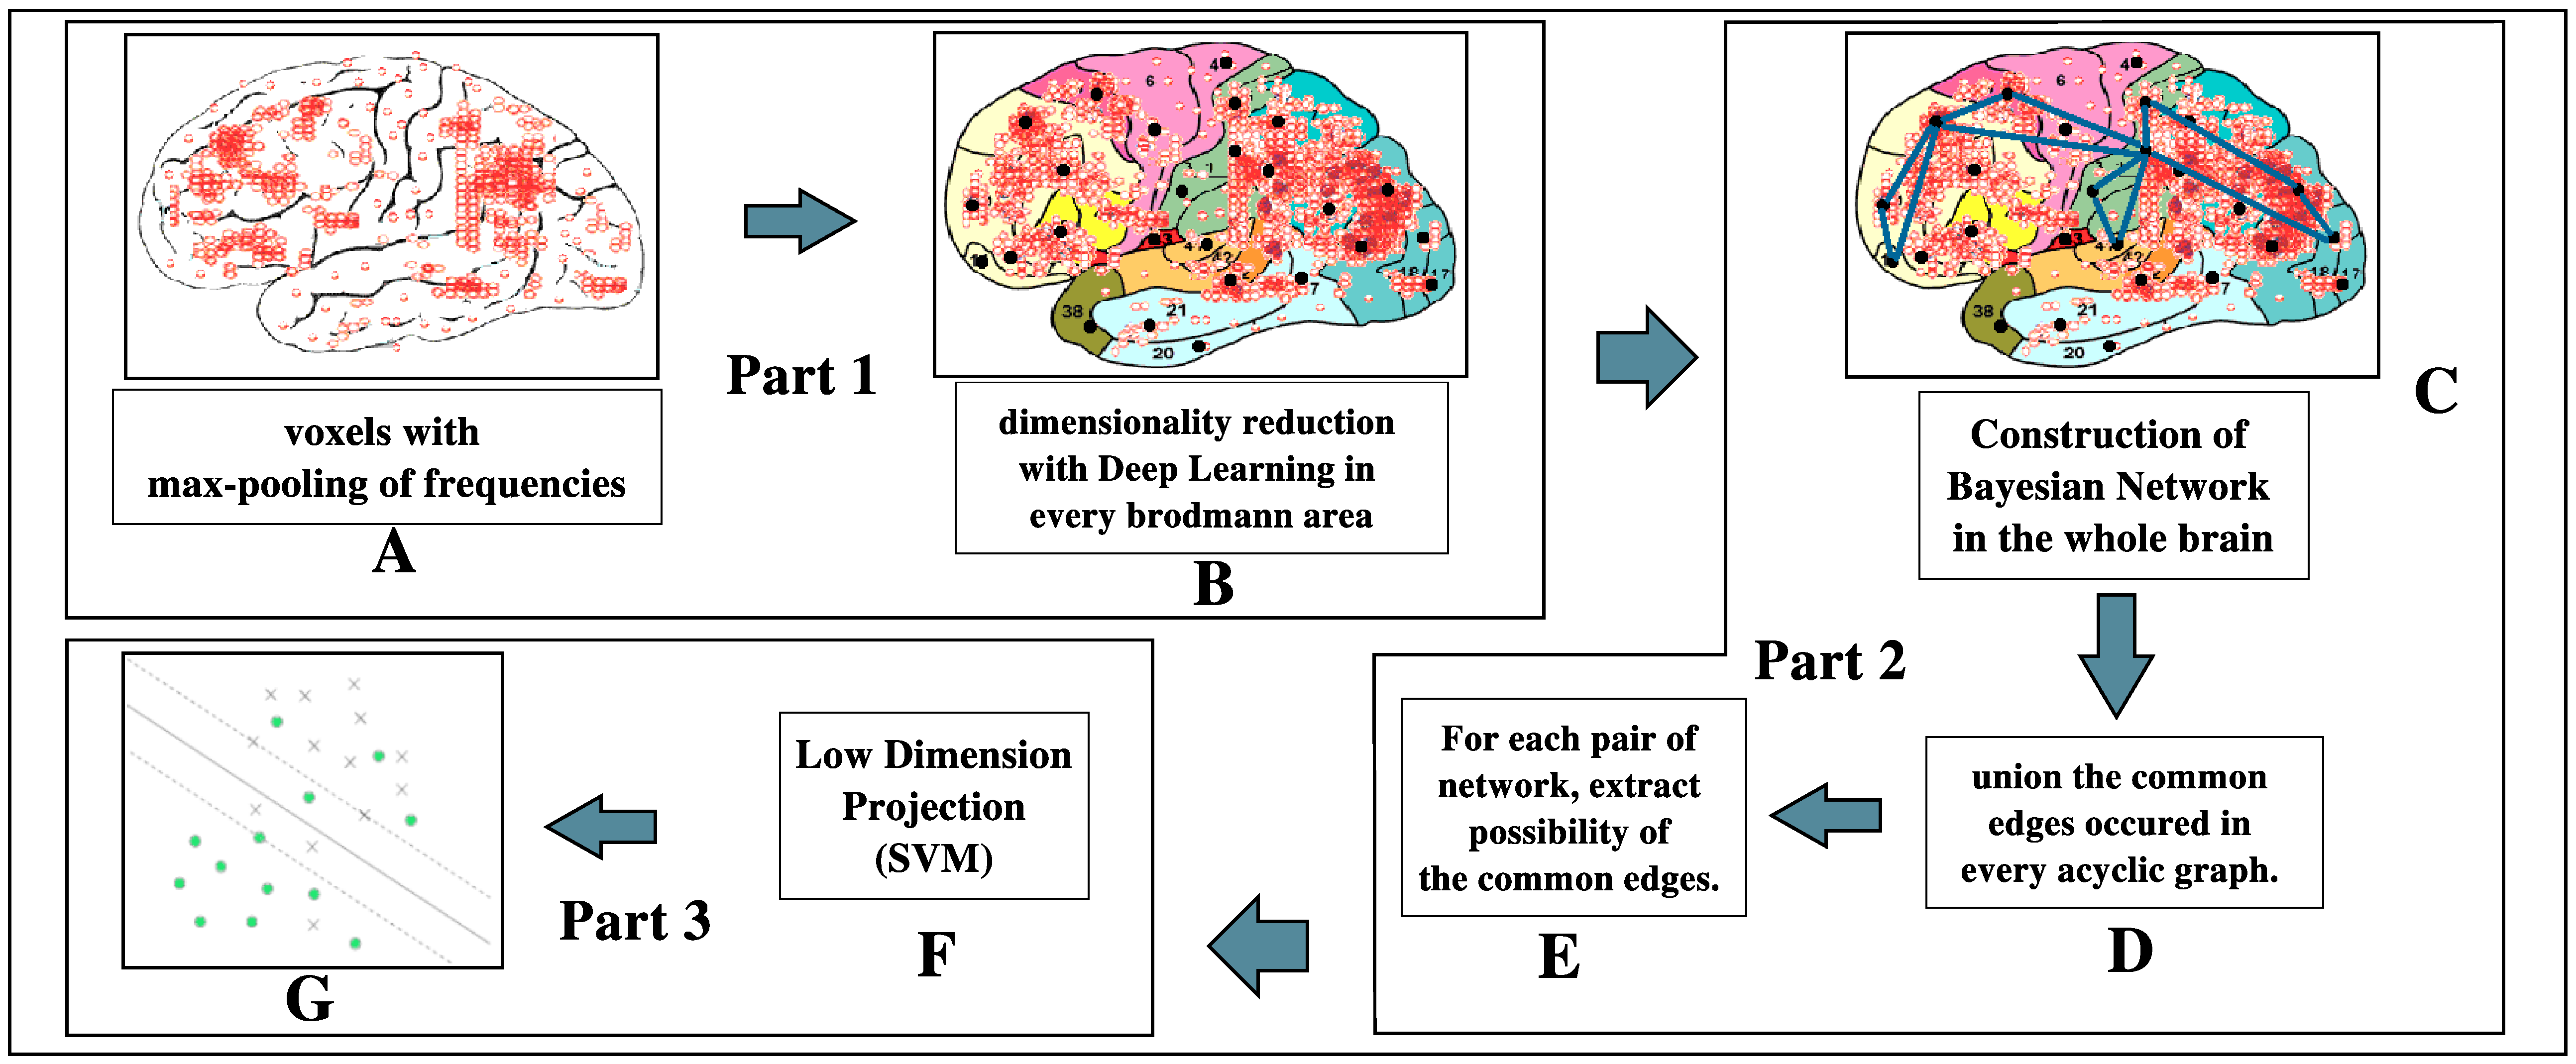
\includegraphics[width=0.9\linewidth]{Figures/overviews.eps}
\end{center}
   \caption{The procedure of Deep Bayesian Network}
\label{fig:overview}
\end{figure*}


However, it will encounter a serious problem during analyzing the ADHD with fMRI data, which are the mass of data and data redundancy. Therefore, dimensionality reduction is essential. Although there are many dimensionality reduction methods proposed, but they only take mathematical requirements into consideration, rather than physical requirements. Luckily, Geoffrey E.Hinton et al.\cite{8} derives a fast, greedy algorithm that can learn deep, directed belief networks one layer at a time, provided the top two layers form an undirected associative memory by using complementary prior.  Because of the good performance in dimensionality reduction currently\cite{7}, Deep Learning has been applied for many areas including image processing\cite{8}\cite{10}, audio classification\cite{9}, natural language processing\cite{12} and so on. Considering its powerful learning ability and advantage of dimensionality reduction and normalization, Deep Learning method will be used to analysis massive fMRI data to dig out the cognitive significance of brain in this paper.


Due to the cause in ADHD cases is unknown, the relationships between different areas should be token into consideration rather than analysis the brain area separately, which meets the requirements of Bayesian network. It is a graphical model that can encode probabilistic relationships among variables of interest. On the one hand, the model can be used to learn causal relationships and gain understanding about a problem domain. For example, in bioinformatics Bayesian network has been used for the interpretation and discovery of gene regulatory pathways\cite{14}. On the other hand, it is an ideal representation for combining prior knowledge and data. Based on these, Bayesian network has been used in information retrieval\cite{15}, natural language processing\cite{16} ,and for the analysis of a medical service's performance for management decisions\cite{17}. In this paper, Bayesian network is applied to retrieval the information between different brain areas, which is shown by the edges in the graph of the Bayesian network.  

 
Figure 1 shows the framework of proposed method. It can be seen that there are totally four steps. The first step is that pre-process the
voxels with max-pooling of frequencies(\textbf{A} in Fig.\ref{fig:overview}). Then, Deep Belief Network is used to reduce dimensionality of data in every brodmann area(\textbf{B} in Fig.\ref{fig:overview}), which reconstructs the different number of voxels in every areas into the same number of features, and the Bayesian network can extract the relationships with the normalized fMRI data(\textbf{C-E} in Fig.\ref{fig:overview}). Finally, using SVM as a classifier to discriminate the ADHD children from normal(\textbf{F-G} in Fig.\ref{fig:overview}). The main contribution of our work is to propose a novel method which combine the dimension-reduced characteristic of Deep Belief Network with the global feature-extracted  characteristic of Bayesian Network. Based on this two characteristics, Deep Belief Network can deal with the huge amount of datas, such as fMRI data. In addition, the features extracted are global, which can represent the whole brain.

The rest of this paper is organized as follows. Section 2 mainly describes the Deep Belief Network method, Bayesian network and the application of two graph model for ADHD data. Section 3 presents our experiments and results on ADHD dataset.

\section{METHOD}
Due to Deep Belief Network and Bayesian Network are two key parts of Deep Bayesian Network we proposed, we will introduce the two methods to you in brief.

\subsection{Deep Belief Network}
Deep Belief Network is made of a stack of
restricted Boltzmann machines(RBM)\cite{13} which is a two-layer, undirected, bipartite graphical model including visible units $v$ and hidden units $h$.


The construction of Deep Belief Network includes
two steps, which are pretraining and back propagation. Pretraining is a down-up unsupervised feature learning. It uses unlabelled data as the input of first RBM layer. After the training in the first layer, the output will act as the input of next layer. Pretraining RBM network make sure that the feature can be mapped into different feature space and keep more feature information at the same time. In each layer, the weights $W$ and biases $a,b$ of the RBM determine the energy of a joint configuration of the hidden and visible units $E(v,h)$,
\begin{equation}
E(v,h;\theta) = -\sum_{i=1}^V \sum_{j=1}^H v_ih_jw_{ij} - \sum_{i=1}^V b_iv_i - \sum_{j=1}^H a_jh_j
\end{equation}
with model parameters $\theta = \{W,b,a\}$ and $v_i,h_j \in \{0,1\}$,$V,H$ represents the number of visible units and hidden units. 


The second step is back propagation, which is a top-down supervised learning. It uses the labelled data to fine-tune the whole network, which spreads the error message $\Delta w_{ij}$ to every level of RBM from the top to down. 
\begin{equation}
\Delta w_{ij} = \epsilon (<v_i,h_j>_{data} - <v_i,h_j>_{recon})
\end{equation}
Where $\epsilon$ is the learning rate and the angle brackets manifests the expectations relative to the distribution specified in the subscript. 
This procedure is viewed as a initialization of parameter weights $W$, which overcome the shortcomings of local optimum and long train time due to random initializtion of parameter weights. compared with RBM, Convolutional Netural Network(CNN) is more popular in field of image recognition\cite{20}\cite{21}. Considering the specificity of fMRI, which is a 4D time series and huge amount of data, we apply a generalized technology deep learning based on RBM other than Convolutional Netural Network(CNN) and autocode.




\subsection{Bayesian Network}
A Bayesian network $B=<N,A,\Theta>$ is a directed acyclic graph (DAG) $<N,A>$ with a conditional probability table (CPT) for each node, collectively represented by $\Theta$. Each node $n \in N$ represents a domain variable $x_i$, and each arc $a \in A$ between nodes represents a probabilistic dependency $p(x_i|x_j)$. The joint probability $p(X)$ can be calculated as follows:
\begin{equation}
p(X) =\prod_{i=1}^m p(x_i |\pi_i))
\end{equation}
where $\pi_i$ denotes the parent $i=1,\cdots,m$ nodes of $x_i$.
There are two major tasks in learning a BN: structure learning and parameters learning. Currently, there are three methods to learn the structure of Bayesian network, which are method based on searching and scoring, method based on testing independence and the mix of two. The third method performs well, especially for Max-Min Hill Climbing(MMHC) algorithm. This paper mainly apply  Max-Min Hill Climbing (MMHC) algorithm to learn structure  efficiently, which can reduce the searching spaces and  improve the learning efficiency of the whole algorithm.





\subsection{The Construction of Deep Bayesian Network}
\subsubsection{Original Idea}
For all our experiments we used the preprocessed rs-fMRI data released for the competition. All the fMRI data volumes are of size $49\times58\times47$ voxels, but the number of samples across time varies among the data capturing centers. For example, there are 172 samples in NYU and 148 samples in KKI. For this huge 4-D fMRI data, large number of calculation is absolutely necessary, which will cause intolerable time consuming. Fortunately, Brodmann divided the cerebral cortex into 52 areas according the brain's cognitive function\cite{22}.  In fact, only 41 brodmann area are used considering some brodmann area possess few voxels. Based on this, we do some research on each brodmann area in order to reduce dimensionality the fMRI data. What is worth mentioning is that variable number in each brodmann area will be normalize to the same size, which achieves the effect of normalization. Deep Belief Network is exact suitable to this. But the performance in single brodmann area is unsteady. some of brodmann areas perform well, such as the areas of 10, 18, 30 etc and some of brodmann areas perform bad, such as the areas of 22, 26, 36, 38 etc. In addition, due to the huge fMRI data, we cann't deal with whole brain data with Deep Belief Network exactly. So we select the performed-well brodmann areas to construct Bayesian Network, to explore the differences in the whole brain between ADHD and normal person. 







\subsubsection{Deep Feature Extraction}
In this paper, the original fMRI data $D$ is a 4-D time series, here we unroll it as this $D=[D_1,\cdots,D_{49\times58\times47}], D_i=[d_1,\cdots,d_{n}], d_i \in R$, $n$ is decided by the data capturing centers. The data $D_i$ is produced by each voxel, which is show in Figure \ref{fig:value}.  The frequency information is quite significant\cite{23}, which can be used as the characteristics of each voxel by the study in our research group. So we select the frequence with the max amplitude as the feature of each voxel by Fast Fourier Transform, which is show in Figure \ref{fig:fre}. 
\begin{equation}
x_i = max(fft(D_i))
\end{equation}

\begin{figure}[ht]
\begin{center}
\subfigure[Value information in each voxel]{
   \label{fig:value}
   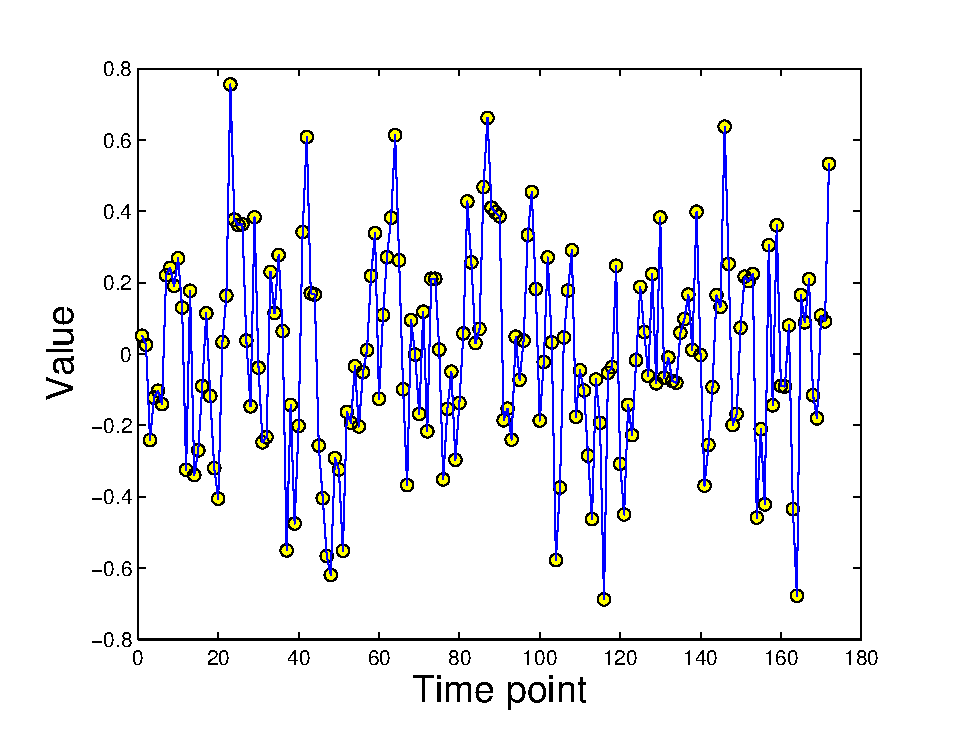
\includegraphics[width=0.8\linewidth]{Figures/voxel_a.eps}}
\subfigure[Frequence information in each voxel]{
   \label{fig:fre}   
   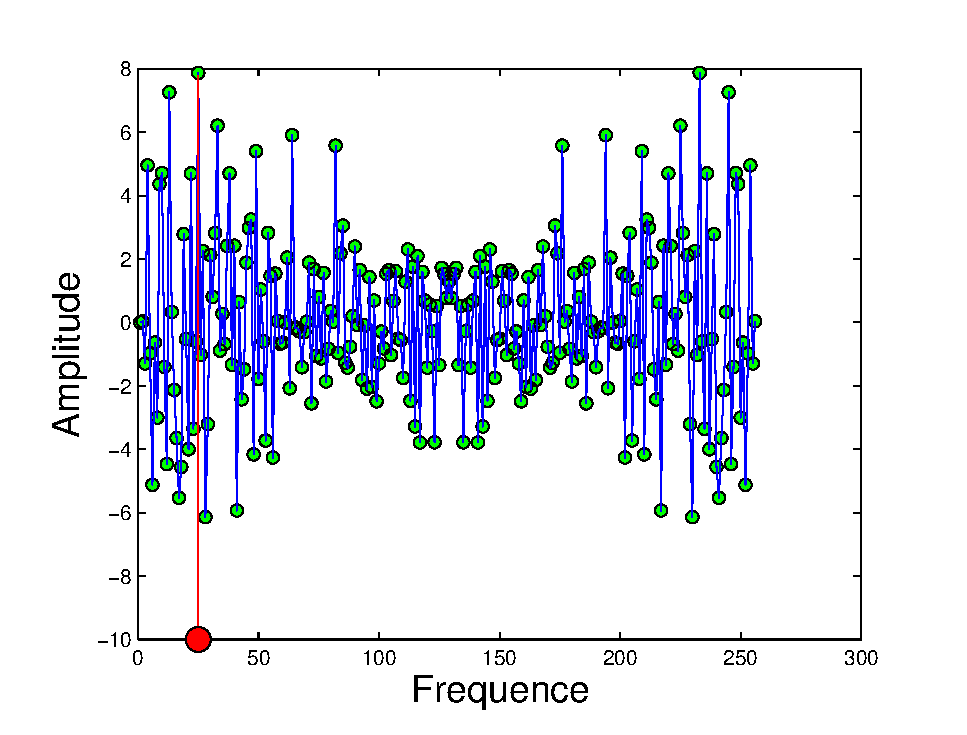
\includegraphics[width=0.8\linewidth]{Figures/voxel_b.eps}}
   \caption{Preprocess in each voxel}
\end{center}
\end{figure}
After that, we divide the dealt data $X=[x_1,\cdots,x_{49\times58\times47}]$ into 41 subsets $X=[X_{m_1},\cdots,X_{m_41}]$ according to Brodmann area which is the input of Deep Belief Network. 



To construct the Deep Belief Network, the forward calculation and backward propagation are needed in every layer.
\begin{eqnarray}
[\theta,X] &=& RBN(X)   \\
\theta  &=& backprop(\theta,X)
\end{eqnarray}
The pseudo-code for application of Deep Belief Network on ADHD data can be seen as following Algorithm \ref{code:DBN} .
\begin{algorithm}[h]
\caption{Deep Feature Extraction}
\label{code:DBN}
\begin{algorithmic}[1]
\Require
original fMRI data $D$

\State Get frequencies with max amplitude in every voxel $x_i$
\[ x_i \gets max(fft(D_i))\]
\State Pre-process frequency information: $X \gets prepro(X_f)$ 
\For{$k \gets 1, 3$} 
\State train the weights $\theta=[w,a,b]$ of single RBM
\[
[\theta,X]\gets RBN(X)
\]
\EndFor
\State Adjust weights with Backpropagation
\[
\theta \gets backprop(\theta,X)
\]
\State Reduce dimensionality:  $Y \gets DBN(\theta,X)$ 
\Ensure
dimensionality-reduced data $Y$
\end{algorithmic}
\end{algorithm}


\subsubsection{Structure Learning of Deep Bayesian Network}
Duo to the reason of ADHD is unknown, it is meaningful to analysis the
dimensionality-reduced data $Y$ and sample label $L$ in the
whole brain with Bayesian Network. First, filter the data $Y$ to wipe out the noise. Second, the MMHC algorithm can speed up the structure of Bayesian network, but it needs the limited parent nodes of each node. So the dependent nodes $I$ are computed by conditional independence testing in filtered data $Y_f$.
\begin{equation}
I = Indep(Y_f)
\end{equation}
Third, we union the limited parent nodes $U$ and use it to learn the structure of all data including training data and testing data. By this, we can get a DAG $G$ and a table $P$ including the information of probability of edge shown in equation below.
\begin{equation}
[G,P] = BN(U,Y_f)
\end{equation}
Forth, the probability of each edge in Bayesian network will be extracted out and viewed as feature $F$ of ADHD children and normal children.


Finally, SVM will be acted as classifier to train the training samples and classify the testing samples, which will get the classified label of testing sample $C$. We choose to use the SVM classifiers for the following reasons. First, the SVM can classify the data points from two classes, which are not easily separable in the feature space, by using a kernel trick to project the data points into a hyperspace where the separation is easy. Second, the SVM regresses the feature space without over fitting on the data by allowing miss classification with a penalty. The accuracy $T$ can be computed by predicted labels $L$ and true labels $Y$. The pseudo-code for application of BN on ADHD data can be seen as following Algorithm \ref{code:BN}.  
\begin{algorithm}[h]
\caption{Structure Learning of Deep Bayesian Network}
\label{code:BN}
\begin{algorithmic}[1]
\Require
dimensionality-reduced data $Y$, labels of data $L$

\State Filter the data: $X_{f} \gets filter(Y)$ 
\State Test Conditional independence
\[
I \gets Indep(X_{f})
\] 
\State union the parent's limitation: $U \gets union(I)$
\State Learning structure of Bayesian Network
\[ [G,P] \gets BN(U,Y_f)
\]
\State Extract feature: $F \gets extract(G,P)$
\State Classify the features: $C \gets svm(F,L)$ 
\State Computer accuracy: $T \gets com(L,C)$ 
\Ensure
accuracy of discrimination $T$
\end{algorithmic}
\end{algorithm}



\section{EXPERIMENTS AND RESULTS}
\subsection{Data}
The data, provided by Neuro Bureau for the ADHD 200 competition, is used for our study. There are eight different centers contributing to the compilation of the whole data set, which makes it diverse as well as complex. In total it consists of 776 training and 197 test subjects. Besides the basic fMRI data, different phenotypic information, such as age, gender, handedness, IQ, is also provided for each subject.


The experimental validations of our proposed method are performed on the training and test data sets of 3 of the data centers - New York University(NYU), Peking University(Peking-1) and Kennedy Krieger Institute(KKI). Consider Table 1 for an overview of the data userd in our study. For NYU, the training subjects are 216, and testing subjects are 41; for Peking-1 dataset, the training subjects are 85, and testing subjects are 50; and for KKI the training subjects and testing subjects are 83 and 11 respectively.


\begin{table}[h]
\label{tab:Information}
\caption{Demographic Information of three Datasets}
\begin{center}
\begin{tabular}{|c|c|c|c|c|c|c|}
\hline
\multirow{3}{*}{type}	& \multicolumn{2}{c|}{NYU} & \multicolumn{2}{c|}{Peking-1} & \multicolumn{2}{c|}{KKI} \\
\cline{2-7}\rule{0pt}{5pt}
					 	& train &  test  & train	& test 	& train & test  \\
						& 216	& 41	  &    85   &   50  &   83   &   11 \\ [2pt]
\hline \rule{0pt}{12pt}
control					& 98	    & 12    &    61   &    27 &   61    &   8 \\
combined					& 73		& 22   &    7    &    9  &   16    &   3 \\
inattentive				& 2		& 0    &    0    &    1  &   5     &   0 \\
hyperactive				& 43		& 7    &    17   &    13 &   1    &   0 \\[2pt]
\hline
\end{tabular}
\end{center}
\end{table}
In compliance with the Health Insurance Portability and Accountability Act(HIPAA) privacy rules, all data used for the experiments of this article are fully anonymized.


\subsection{The Experiment of Parameter Design}
To construct a Deep Bayesian Network, we must set up the number of network nodes, which is equal to selected brodmann areas. If the value of number is small, Bayesian network will not extract the enough information of relationships between brain areas. If the value of number is too large, the probability that the unrelated brain areas will be chose as a node will get higher, which has a side effect on the final classification. In addition,  with the increase of the variables, the search space of network structure will present exponentially. So the experiment of parameter designing is significant.
\subsubsection{Parameter Design}
As NYU dataset in the ADHD-200 competition achieved the lowest discrimination results, Deep Belief Network is particularly tested on the NYU dataset of 41 areas and softmax as a classifier generates the accuracies of different brain areas,which is convenient for the choice of node in the Bayesian network. The results of 41 regions are shown in Figure~\ref{fig:NYU}.
\begin{figure}[ht]
\begin{center}
\subfigure[Accuracy of NYU in 41 Areas]{
   \label{fig:NYU}
   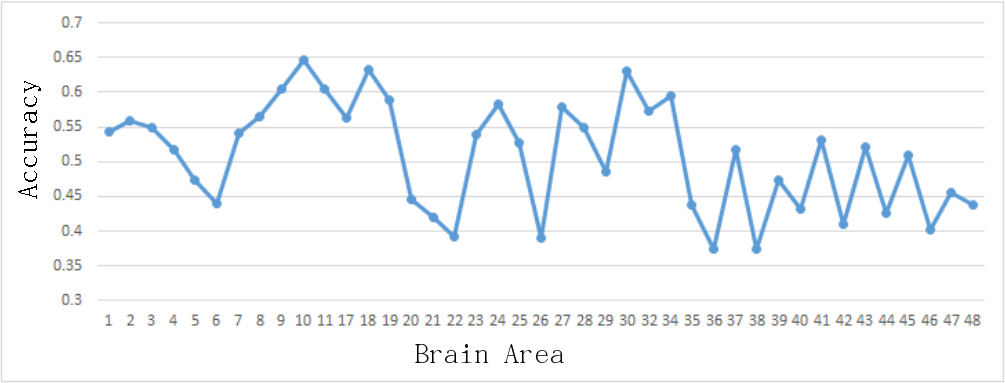
\includegraphics[width=0.8\linewidth]{Figures/NYU.png}}
\subfigure[Accuracy in Different Number of Brain Areas]{
   \label{fig:BN}   
   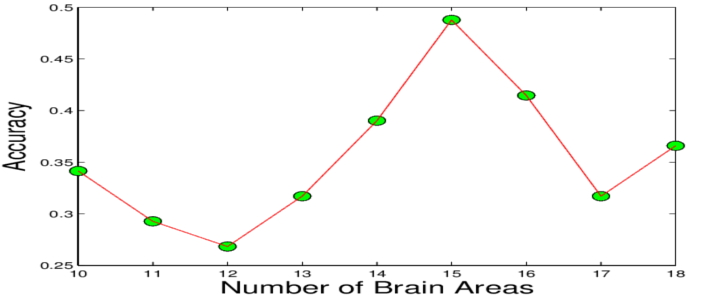
\includegraphics[width=0.9\linewidth]{Figures/BN.png}}
   \caption{Parameter Design in NYU dataset}
\end{center}
\end{figure}


From Figure~\ref{fig:NYU}, we can see that different brain areas have different performance of discrimination. The areas of 10, 18, 30, 9, 11, 19, 34, 32, 8, 17, 2, 28, 3, 1, 7, 23, 25, 41 perform well. According to brodmann definition, it is clear that prefrontal cortex(9,10,25), visual cortex(8,17,18,19), somatosensory cortex(1,2,3,7) and cingulate cortex(23,30,32) is related to the ADHD closely. Therefore, they are selected as the input of Bayesian Network.  The Figure ~\ref{fig:BN} shows that the accuracy of discriminate fluctuate a little from 10 to 18, but it reaches the peak when the number of brain areas is equal 15. So we will choose 15 brain areas in the front to construct the Bayesian network. Besides, using the relationships between brain areas to discriminate ADHD is better than using information in single brain area and the best result in  ADHD-200 competition.


\subsection{Performances on NYU, Peking-1 and KKI dataset}
The same experiments are excuted on the NYU, Peking-1 and KKI dataset. The results released by ADHD-200 competition are 35.19\% for NYU, 51.05\% for Peking-1 and 61.90\% for KKI respectively. The prediction accuracies of Attributed graph distance\cite{19} (AGD) are none, 58.82\%,54.55\%. The Deep Bayesian Network  gains a higher prediction accuracies than Deep Belief Network single, which are 48.78\% for NYU, 54.00\% for Peking-1 and 72.72\% for KKI. The details show in Figure ~\ref{fig:dataset}.
\begin{figure}[ht]
\begin{center}
%\fbox{\rule{0pt}{2in} \rule{0.9\linewidth}{0pt}}
   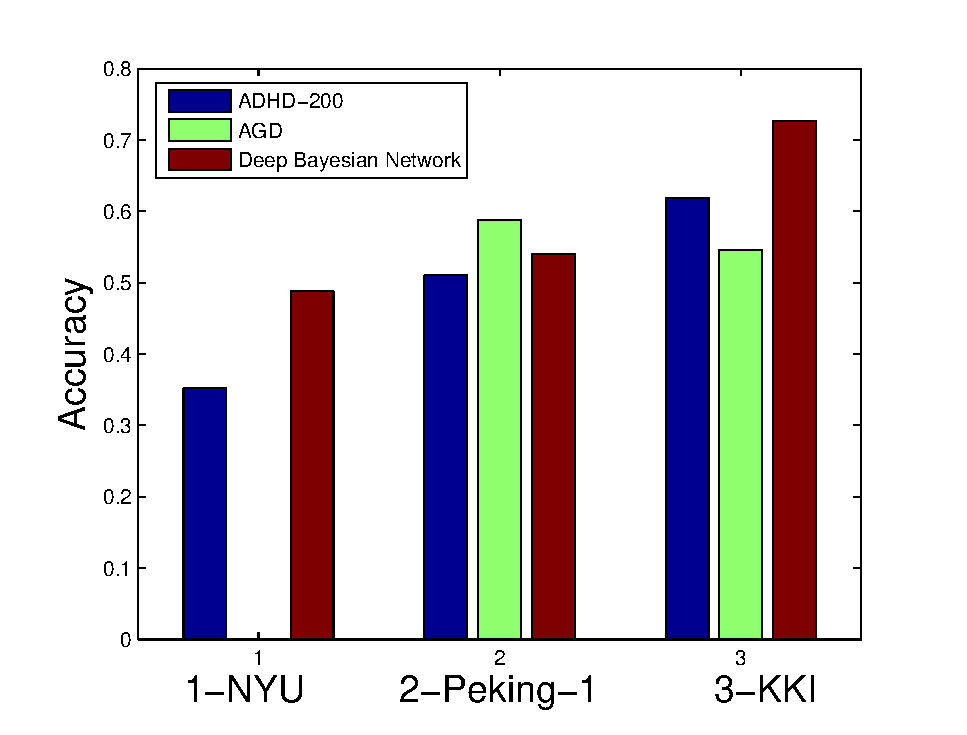
\includegraphics[width=0.8\linewidth]{Figures/Datasets.eps}
\end{center}
   \caption{Performance in Different Datasets}
\label{fig:dataset}
\end{figure}


From this chart, we can see that Deep Bayesian Network improves the prediction accuracies  in these three datasets  compared with the results of ADHD-200 competition. Besides, the increase of accuracy is the highest in the NYU dataset than other two datasets. The different number of training samples have a big effect on the accuracy. This effect is shown in Figure ~\ref{fig:Number}.
\begin{figure}[ht]
\begin{center}
%\fbox{\rule{0pt}{2in} \rule{0.9\linewidth}{0pt}}
   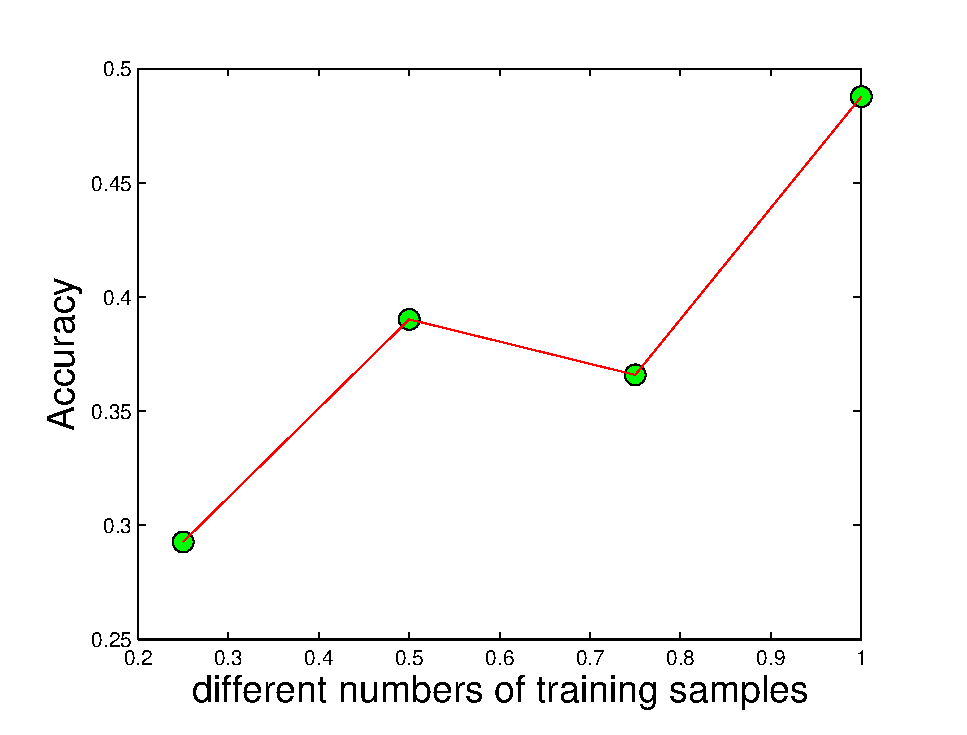
\includegraphics[width=0.8\linewidth]{Figures/Number.eps}
\end{center}
   \caption{Performance in Different Number of training samples}
\label{fig:Number}
\end{figure}



To verify generality of our method, we make another experiment, which is described as follow. First, we mix the training dataset and the testing dataset in the ADHD-200 competition. Second, we randomly select same number of training dataset in the competition. Third, the left dataset will be acted as testing dataset to check the performance by Deep Bayesian Network method. we repeat the three steps above for 100 times, the detail information is show in Tab 2. Considering that discriminating the ADHD is important and meaningful, we take the prediction accuracy of the method along with the specificity and sensitivity values into consideration.

%NYU			&  -		&   -	 &  - &  64.65	&  68.77 & 43.89 \\[2pt]
%Peking-1		& 58.82		&  92.59 	& 20.83 & 66.32 & 87.71 &22.88\\[2pt]
%KKI			& 54.55		& 62.50	& 33.33 & 58.96  & 82.98  & 55.56\\[2pt]


\begin{table}[h]
\label{tab:2}
\caption{The Detail information in Different Datasets}
\begin{center}
\begin{tabular}{cccc}
\hline

Dataset  	&   Accuracy  	&	Specificity  &	Sensitivity \\
\hline
NYU			&  64.7	&  68.8 & 43.9 \\[2pt]
Peking-1		& 66.3 & 87.7 &22.9\\[2pt]
KKI			& 59.0  & 83.0  & 55.6\\[2pt]
\hline
\end{tabular}
\end{center}
\end{table}


Although the data in Tab 2 have no comparison with the results in the ADHD-200 competition, the generality of our method is good.




%------------------------------------------------------------------------
\section{CONCLUSION}
In this paper, a novel method called Deep Bayesian Network, is proposed to classify fMRI ADHD image data. Because of the combination Deep Belief network and Bayeisan network, Deep Bayesian Network can compute relationships among brodmann brain areas more effectively. A series of experimental results also prove that Deep Bayesian network  improves the classification performatnce of ADHD greatly comparing with the ADHD-200 competition resutls. 


In the future, we could find more effective method to choose the different brain areas as the input of Bayesian Network. In addition, the distance between different brain areas is different, so they have different influence over each other. we could take  the area's neighborhood into consideration manually to strengthen the structure learning.



%-------------------------------------------------------------------------
\section{ACKNOWLEDGMENT}

This work was supported by National Natural Sciences
Foundation of China (No.61272267, 61270220, 51075306,
61273261), Program for New Century Excellent Talents in
University (NCET-11-0381), Fundamental Research Funds for
the Central Universities, State Key Laboratory of Software
Engineering.

{\small
\bibliographystyle{ieeetr}
\bibliography{egbib}
}

\end{document}
